\subsection{Skiplist}
\label{Sec-Transactions-SkipList}

The Single-Writer-Multi-Readers lock used to synchronize the sequential and the parallel skiplists complicates the priority queue design and adds overhead. In this section, we explore an alternative design using hardware transactions. 
However, the naive approach of making all operations transactional causes too many aborts. Instead, the server increments a timestamp whenever a head-moving operation - \texttt{SL::moveHead()} or \texttt{SL::chopHead()} - starts or finishes. A \texttt{SL::addPar()} operation first reads the timestamp and executes a nontransactional \texttt{SL::find()} and then starts a transaction for the actual insertion, adding the server's timestamp to its read set and aborting if it is different from the initially recorded value. Moreover, if the timestamp changes after starting the transaction, indicating a head-moving operation, the transaction will be aborted due to the timestamp conflict.  
If the timestamp is valid, \texttt{SL::find()} must have recorded the predecessors and successors of the new bucket at each level $i$ in \texttt{preds[i]} and \texttt{succs[i]}, respectively. If a bucket already exists, the counter is incremented inside the transaction and the operation completes. If the bucket doesn't exist, the operation proceeds to check if \texttt{preds[i]} points to \texttt{succs[i]} for all levels $0 \le i \le \maxLvl$. If so, the pointers have not changed before starting the transaction and the new bucket can be correctly inserted between \texttt{preds[i]} and \texttt{succs[i]}. Otherwise, we commit the (innocuous) transaction, yet restart the operation.


%%%%%%%%%%%%%%%%%%%%%%%%5

%In the \texttt{SL::addPar()} operation, we initially tried to include our \texttt{SL::find()} inside a transaction, together with the \emph{mutable} operations, those that perform pointer changes or that increment counters. However, we were having too many aborts caused by a poor interaction of mutable interactions and the finds. We finally decided to use an approach similar to the one in the lock-based implementation: our \texttt{SL::find()} first executes outside a transaction, and then \texttt{SL::addPar()} starts a transaction. The function proceeds to check a timestamp indicating whether a head-moving operation took place.

%If the timestamp is valid, \texttt{SL::find()} returned the predecessor and successor of the newly inserting bucket at each level $i$ in \texttt{preds[i]} and \texttt{succs[i]}, respectively. If a bucket is found, the counter is incremented inside the transaction and the operation finishes. Otherwise, the operation proceeds to check if \texttt{preds[i]} points to \texttt{succs[i]} for all levels $0 \le i \le \maxLvl$. If that happens, indicating that the pointers did not change before acquiring the transaction, the new bucket is inserted between \texttt{preds[i]} and \texttt{succs[i]} for all levels $0 \le i \le \maxLvl$. In the negative case, we commit the (innocuous) transaction, yet restart the operation.

%The head-moving operations (\texttt{SL::moveHead()} and \texttt{SL::chopHead()}) increment the timestamp when they start executing and when they finish executing. 
%This way, they are able to interrupt inserting \texttt{SL::addPar()}s in the parallel part in a very natural manner: when the timestamp associated with these operations moves, the transactions are immediately aborted as the timestamp is in their read set.

%%%%%%%%%%%%%%%%

Figures~\ref{fig:tsx1} and~\ref{fig:tsx2} compare the performance of the lock-based implementation and the implementation based on hardware transactions for two different percentages of \texttt{PQ::add()}s and \texttt{PQ::removeMin()}s. When fewer \texttt{PQ::removeMin()} operations are present, the timestamp changes less frequently and the \texttt{PQ::add()} transactions are aborted fewer times, which increases performance  in the 80\%-20\% insertion-removal mix. In the $50\%$-$50\%$ mix, we obtain results comparable to the \emph{pqe} algorithm using the lock-based approach, albeit with a much simpler implementation.

\begin{figure}[htb]
\centering
\begin{minipage}{.495\textwidth}
	\centering
  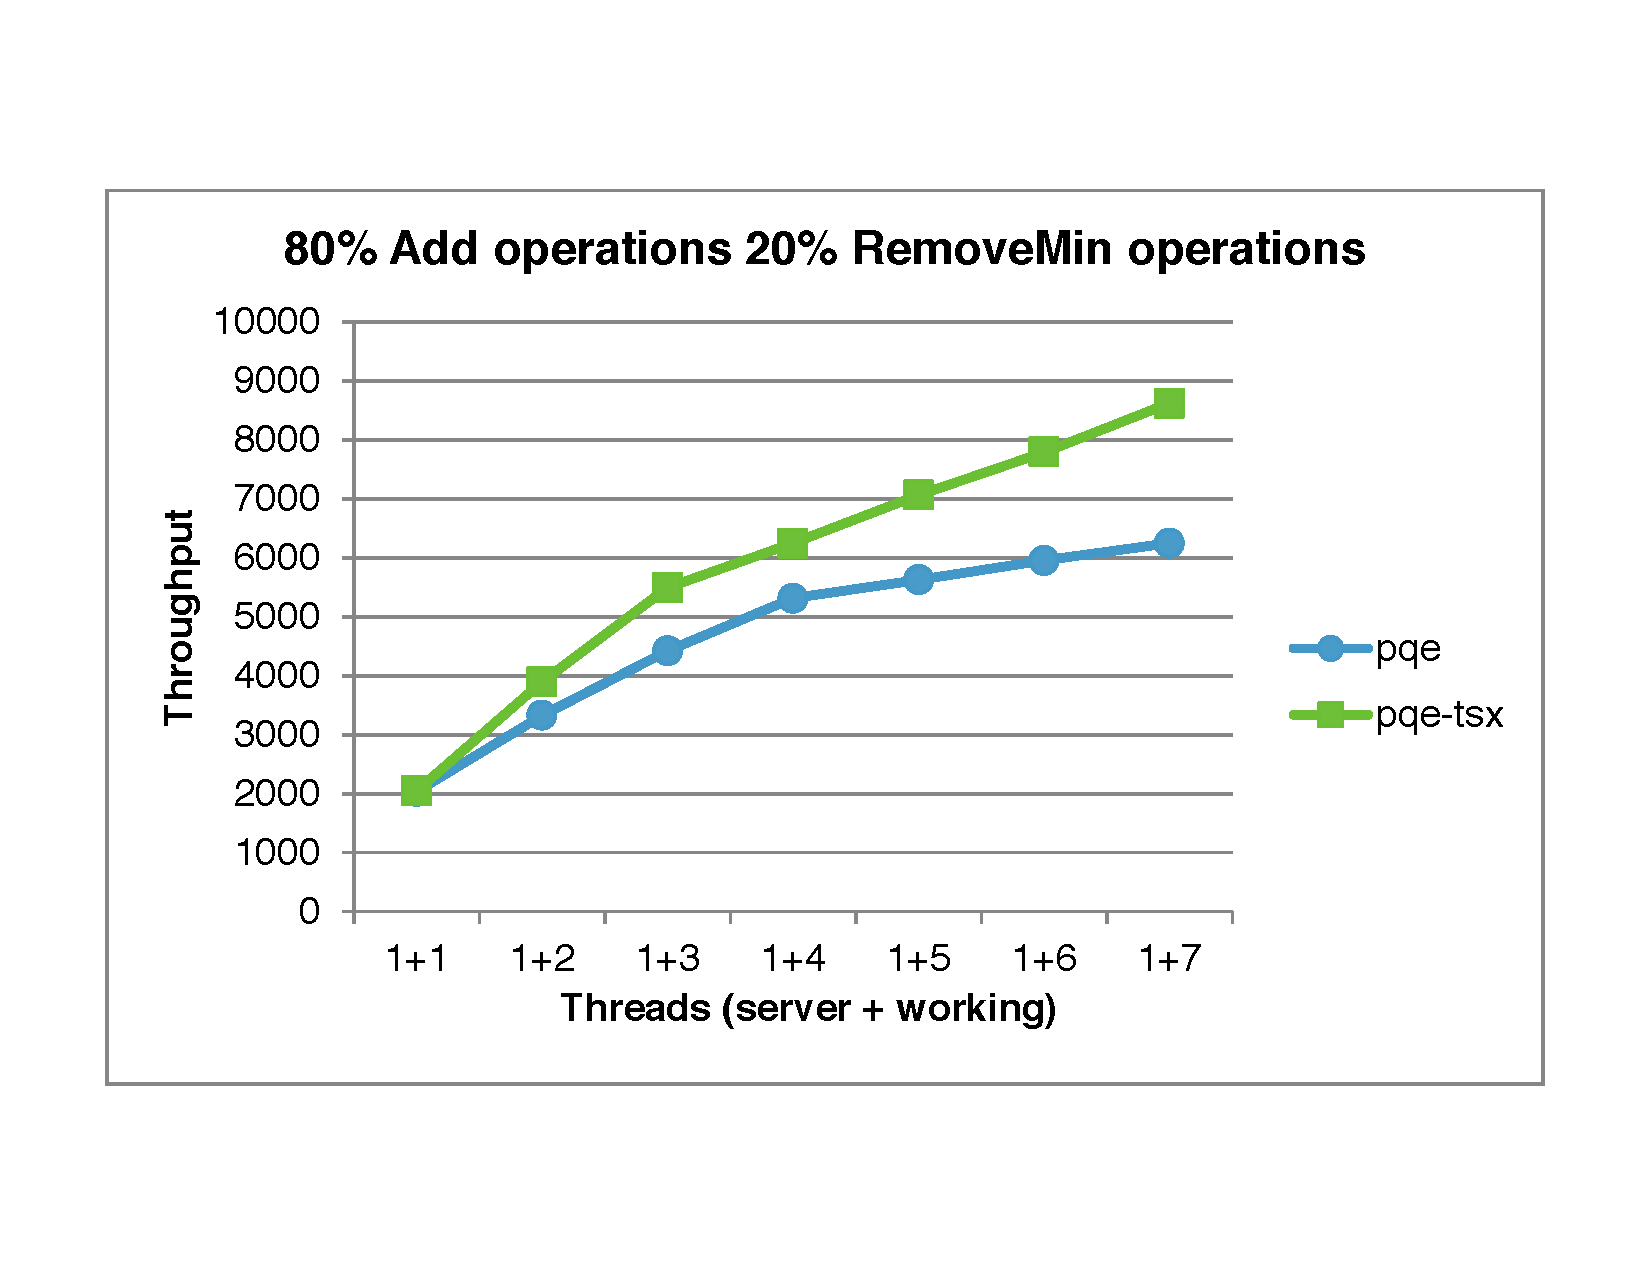
\includegraphics[width=\linewidth]{img/tsx-80-20.pdf}
\caption{Priority queue performance when we use a transaction-based dual skiplist; 80\% \texttt{add()}s, 20\% \texttt{removeMin()}s.}
\label{fig:tsx1}
\end{minipage}%
\hfill%
\begin{minipage}{.495\textwidth}
	\centering
  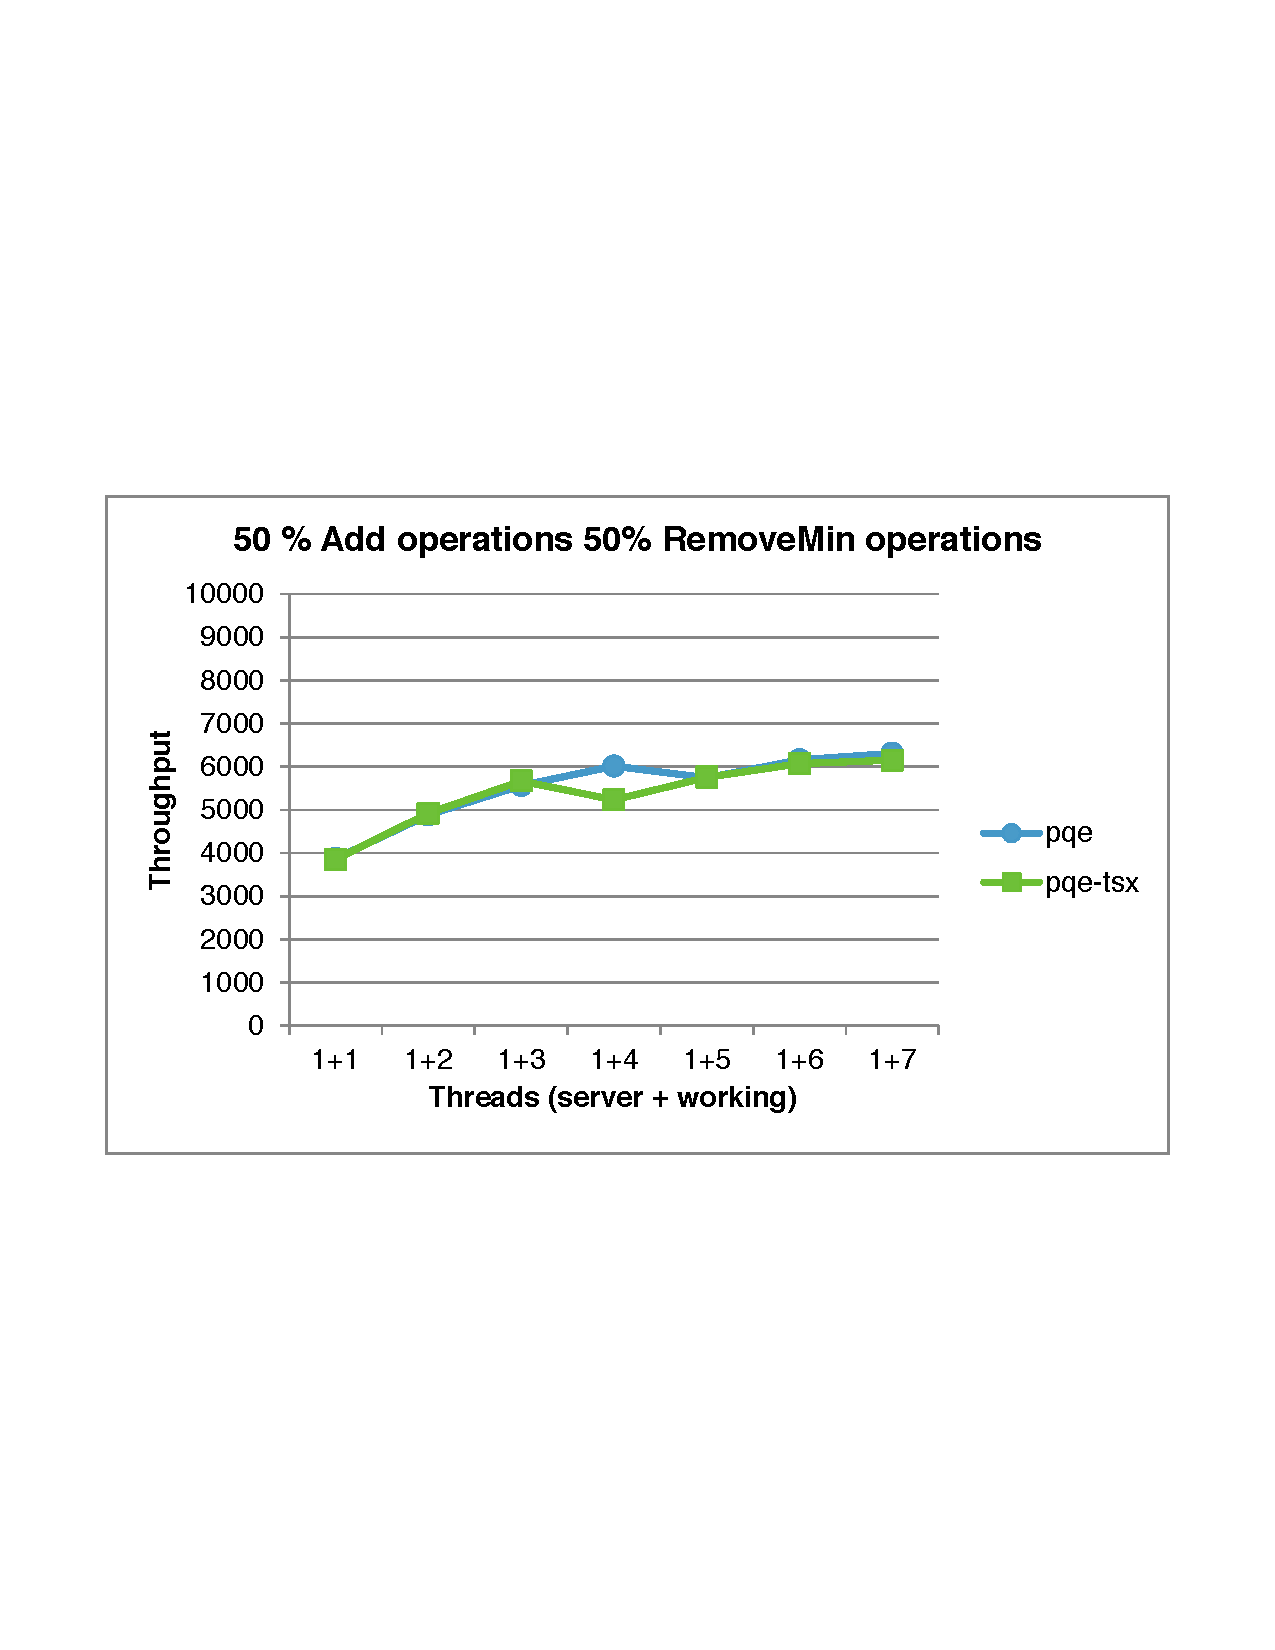
\includegraphics[width=\linewidth]{img/tsx-50-50.pdf}
\caption{Priority queue performance when we use a transaction-based dual skiplist; 50\% \texttt{add()}s, 50\% \texttt{removeMin()}s.}
\label{fig:tsx2}
\end{minipage}
\end{figure}
